\section{}
\textit{Modify a MATLAB script provided on eClass with the derived coefficients. Solve the problem with the modified code for two different Peclet numbers equal to 0.1 and 100 using N = 100. Compare the numerical results to the analytical solution, which is}
\[
    T(x) = \frac{\exp(\text{Pe} \cdot x) - 1}{\exp(\text{Pe}) - 1}
\]
\textit{Plot numerical and analytic distribution on two different plots corresponding to different Peclet numbers. Explain the results. Calculate a maximum absolute error for each Peclet number.} \\
\begin{figure}[H]
    \centering
    \begin{subfigure}{0.7\textwidth}
        \centering
        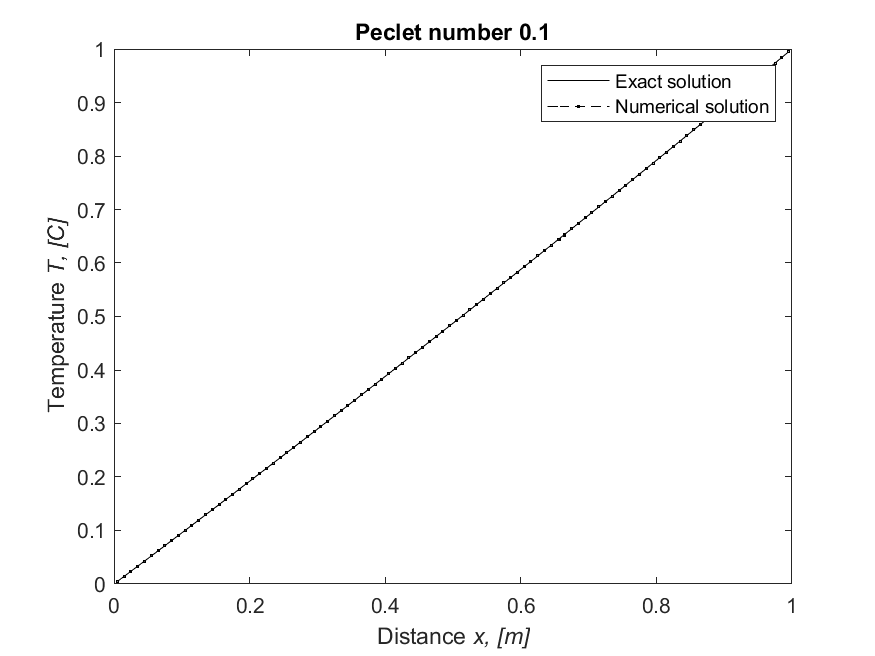
\includegraphics[width=\textwidth]{Questions/Code/peclet_0.1.png}
        \caption{Peclet number = 0.1}
    \end{subfigure}
    \begin{subfigure}{0.7\textwidth}
        \centering
        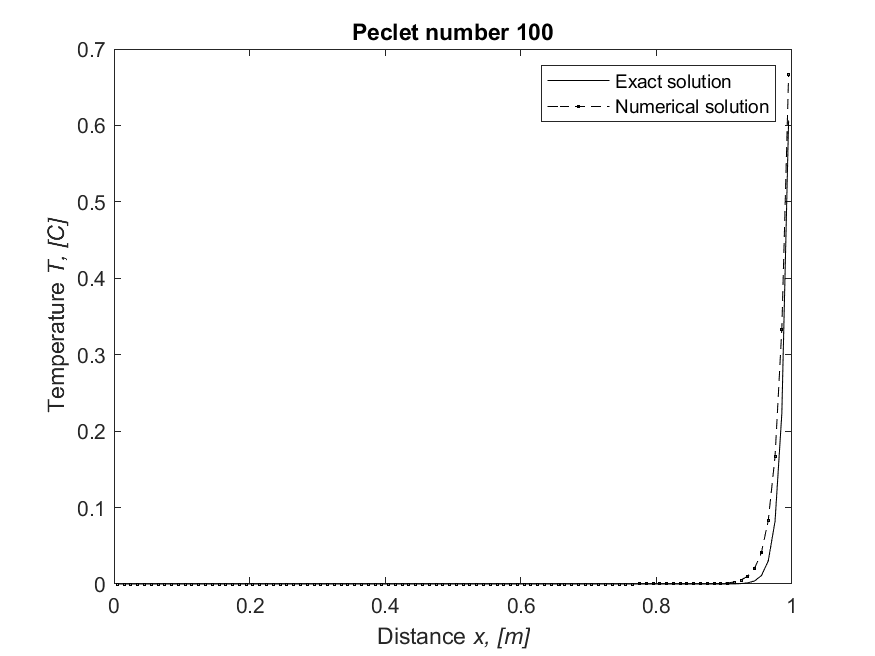
\includegraphics[width=\textwidth]{Questions/Code/peclet_100.png}
        \caption{Peclet number = 100}
    \end{subfigure}
    \caption{Analytical and numerical solutions for Peclet number = 0.1 and 100}
\end{figure}
\begin{figure}[H]
    \centering
    \begin{subfigure}{0.7\textwidth}
        \centering
        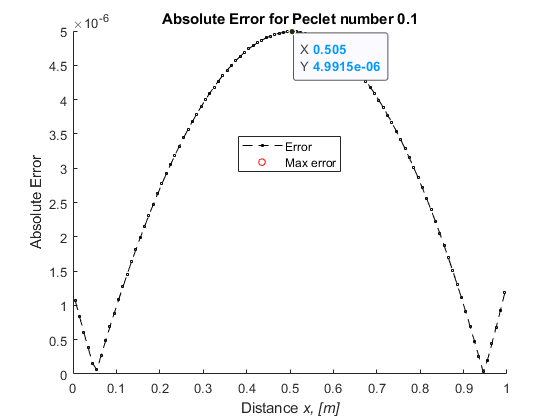
\includegraphics[width=\textwidth]{Questions/Code/error_0.1.png}
        \caption{Peclet number = 0.1}
    \end{subfigure}
    \begin{subfigure}{0.7\textwidth}
        \centering
        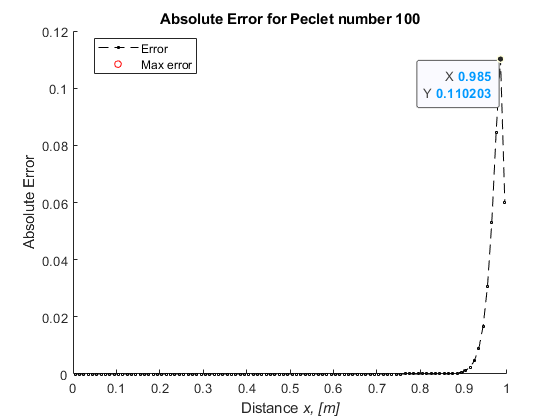
\includegraphics[width=\textwidth]{Questions/Code/error_100.png}
        \caption{Peclet number = 100}
    \end{subfigure}
    \caption{Absolute error for Peclet number = 0.1 and 100}
\end{figure}
% can you expand more on why small rate of diffusion leads to smooth temperature distribution and large rate of convection leads to steep temperature distribution?
Peclet number is the ratio between the rate of convection and the rate of diffusion. When the Peclet number is small, the rate of diffusion is much larger than the rate of convection. This means that the temperature distribution is dominated by the diffusion term. As a result, the temperature distribution is smooth and the temperature gradient is small. 

When the Peclet number is large, the rate of convection is much larger than the rate of diffusion. This means that the temperature distribution is dominated by the convection term. As a result, the temperature distribution is steep and the temperature gradient is large. 

The numerical solution is in good agreement with the analytical solution for both Peclet numbers. The maximum absolute error for Peclet number = 0.1 is $5$E-6 and the maximum absolute error for Peclet number = 100 is 0.11. 

A finer mesh is required to capture the steep temperature distribution for Peclet number = 100.\\

\lstinputlisting[language=Matlab]{Questions/Code/convdiff_CD.m}